En esta sección se detallarán los casos de uso del sistema.  Para facilitar la lectura, los casos de uso y escenarios se agruparán por subsistemas.

Cada caso de uso tendrá la siguiente información:
\begin{itemize}
\item Nombre.  Nombre que permita identificar al caso de uso.
\item Precondiciones.  Las precondiciones indican una situación que es de obligado cumplimiento antes del caso de uso.  Por simplicidad, las precondiciones se omitirán en los casos de uso en los que no existan.
\item Descripción.  La descripción indica de forma resumida la finalidad del caso de uso.
\item Actores.  Los actores serán todos aquellos posibles participantes en el caso de uso.
\item Escenario principal.  El escenario principal indica de forma ordenada los pasos que se realizan en el caso de uso.
\item Escenarios alternativos.  Los escenarios alternativos representan variaciones o divergencias respecto al escenario principal.  Por simplicidad, los escenarios alternativos se omitirán en los casos de uso en los que no existan.
\end{itemize}


\subsection{Subsistema de gestión de usuarios}
\label{casos_uso_subsistema_usuarios}
En esta sección se detallarán los casos de uso y escenarios pertenecientes al subsistema de gestión de usuarios.
La figura \ref{fig:casos_uso_subsistema_usuarios} muestra el diagrama de casos de dicho subsistema.

\begin{figure}[h]
\centering
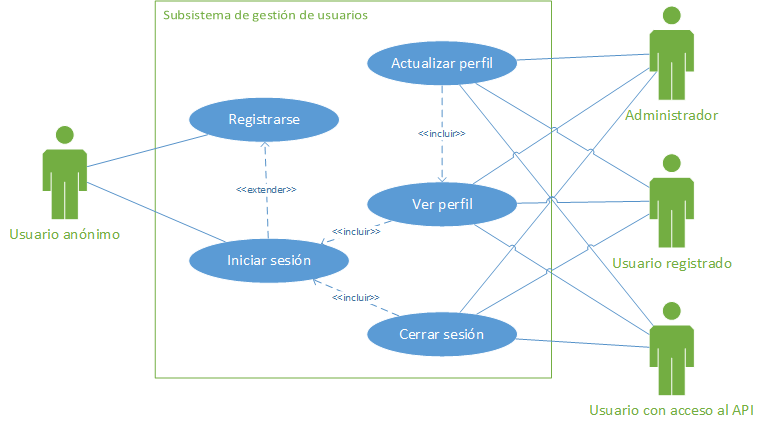
\includegraphics[width=\textwidth]{casos_uso_usuarios.png}
\caption{Diagrama de casos de uso del subsistema de gestión de usuarios}
\label{fig:casos_uso_subsistema_usuarios}
\end{figure}


\subsubsection{Caso de uso ``registrarse''}
\begin{description}
\item[Descripción] 				El usuario no dispone de una cuenta en el sistema y quiere crear una.
\item[Actores]					Cualquier usuario anónimo.
\item[Escenario principal]	 	\hfill
								\begin{enumerate}
								\item El usuario accede al formulario de registro.
								\item Una vez en el formulario de registro, el usuario rellena todos los campos requeridos.
								\item Si el usuario lo decide también puede rellenar los campos opcionales.
								\item Tras rellenar los campos el usuario pulsa el botón de registro.
								\item El sistema guarda los datos y crea la nueva cuenta de usuario con estado bloqueado.
								\end{enumerate}
\item[Escenario alternativo 1]	El usuario no rellena todos los campos necesarios.
								\begin{enumerate}
								\item Cuando el usuario pulse el botón para completar el registro el sistema notificará del error.
								\item Se continuará desde el punto 2 del escenario principal.
								\end{enumerate}
\item[Escenario alternativo 2]	El nombre de usuario ya existe en el sistema.
								\begin{enumerate}
								\item Cuando el usuario pulse el botón para completar el registro el sistema notificará del error.
								\item Se continuará desde el punto 2 del escenario principal.
								\end{enumerate}
\item[Escenario alternativo 3]	El email de usuario ya existe en el sistema.
								\begin{enumerate}
								\item Cuando el usuario pulse el botón para completar el registro el sistema notificará del error.
								\item Se continuará desde el punto 2 del escenario principal.
								\end{enumerate}
\end{description}


\subsubsection{Caso de uso ``activar usuario''}
\begin{description}
\item[Descripción] 				El administrador activa una cuenta de un usuario para que éste pueda utilizarla.
\item[Actores]					El administrador del sistema.
\item[Precondiciones]			La cuenta de usuario debe ser registrada previamente en el sistema.
\item[Escenario principal]	 	\hfill
								\begin{enumerate}
								\item El administrador accede al panel de administración.
								\item Una vez en el panel de administración, accede a la vista de usuarios.
								\item El administrador selecciona el usuario o usuarios a activar.
								\item Pulsa el botón correspondiente para activar los usuarios.
								\item El sistema actualiza el estado de los usuarios y permite que inicien sesión en el sistema.
								\end{enumerate}
\end{description}


\subsubsection{Caso de uso ``iniciar sesión''}
\begin{description}
\item[Descripción] El usuario accede al sistema utilizando su nombre de usuario y contraseña.
\item[Actores] Cualquier usuario anónimo.
\item[Precondiciones] La cuenta de usuario con la que se inicia sesión ha sido activada por un administrador.
\item[Escenario principal] \hfill
						 	\begin{enumerate}
							\item El usuario accede al formulario de inicio de sesión
							\item El usuario introduce su nombre de usuario
							\item El usuario introduce su contraseña
							\item El usuario inicia sesión pulsando el botón correspondiente
							\end{enumerate}
\item[Escenario alternativo 1] El usuario no existe
							\begin{enumerate}
							\item El sistema notificará al usuario de que el nombre de usuario introducido no existe
							\item Se continuará desde el paso 2 del escenario principal
							\end{enumerate}
\item [Escenario alternativo 2] La contraseña es incorrecta
							\begin{enumerate}
							\item El sistema notificará al usuario de que la contraseña introducida es incorrecta
							\item Se continuará desde el paso 2 del escenario principal
							\end{enumerate}							
\end{description}


\subsubsection{Caso de uso ``cerrar sesión''}
\begin{description}
\item[Descripción] 			El usuario quiere cerrar su sesión en el sistema.
\item[Actores] 				Administrador, usuario registrado o usuario con capacidad de acceso al API.
\item[Precondiciones]  		Haber iniciado sesión en el sistema
\item[Escenario principal] 	\hfill
						 	\begin{enumerate}
							\item El usuario con sesión iniciada pulsa en el botón para cerrar sesión.
							\item El sistema redirige al usuario a la vista principal con la sesión ya cerrada.
							\end{enumerate}							
\end{description}


\subsubsection{Caso de uso ``ver perfil''}
\begin{description}
\item[Descripción] 			El usuario quiere ver la información sobre su cuenta almacenada en el sistema.
\item[Actores] 				Administrador, usuario registrado o usuario con capacidad de acceso al API.
\item[Precondiciones]  		Haber iniciado sesión en el sistema
\item[Escenario principal] 	\hfill
						 	\begin{enumerate}
							\item El usuario con sesión iniciada pulsa en el botón para ver su información.
							\item El sistema muestra una vista de la cuenta del usuario con todos los datos almacenados.
							\end{enumerate}
\item[Escenario alternativo 1] El usuario cuenta con capacidad de acceso al API
							\begin{enumerate}
							\item Similar al escenario principal, pero el sistema mostrará también el \textit{token} de acceso al API.
							\end{enumerate}
\item [Escenario alternativo 2] Acceso a un perfil no propio.
							\begin{enumerate}
							\item El usuario pulsa en el perfil de otro usuario del sistema.
							\item El sistema muestra una vista de la cuenta de usuario.
							\item El sistema no muestra en ningún caso el \textit{token} de acceso al API.
							\end{enumerate}							
\end{description}


\subsubsection{Caso de uso ``actualizar perfil''}
\begin{description}
\item[Descripción] 			El usuario quiere modificar la información almacenada en el sistema sobre su cuenta.
\item[Actores] 				Administrador, usuario registrado o usuario con capacidad de acceso al API.
\item[Precondiciones]  		Haber iniciado sesión en el sistema
\item[Escenario principal] 	\hfill
						 	\begin{enumerate}
							\item El usuario con sesión iniciada pulsa en el botón para ver su información.
							\item Una vez en la vista del perfil, el usuario pulsa el botón para modificar su información.
							\item El usuario modifica los datos que considere necesarios.
							\item El usuario introduce su contraseña actual para asegurar su identidad.
							\item El sistema actualiza la información de la cuenta de usuario.
							\end{enumerate}
\item[Escenario alternativo 1] La contraseña actual no es válida.
							\begin{enumerate}
							\item El sistema informará al usuario de su error y no modificará la información almacenada.
							\item Se continua desde el punto 3 del escenario principal.
							\end{enumerate}
\item [Escenario alternativo 2] El usuario quiere modificar su contraseña.
							\begin{enumerate}
							\item El usuario debe introducir su nueva contraseña dos veces para evitar errores.
							\item Se continua desde el punto 4 del escenario principal.
							\end{enumerate}							
\item [Escenario alternativo 3] Las nuevas contraseñas no coinciden.
							\begin{enumerate}
							\item Las nuevas contraseñas introducidas no coinciden.
							\item El sistema informa al usuario del error.
							\item Se continua desde el punto 1 del escenario alternativo 2.
							\end{enumerate}							
\item[Escenario alternativo 4] El nuevo correo es inválido o ya existe en el sistema.
							\begin{enumerate}
							\item El sistema informará al usuario de su error y no modificará la información almacenada.
							\item Se continua desde el punto 3 del escenario principal.
							\end{enumerate}							
\end{description}

\subsection{Subsistema de gestión de debates}
\label{casos_uso_subsistema_debates}
En esta sección se detallarán los casos de uso y escenarios pertenecientes al subsistema de gestión de debates.
La figura \ref{fig:casos_uso_subsistema_debates} muestra el diagrama de casos de uso del subsistema de gestión de debates.

\begin{figure}[h]
\centering
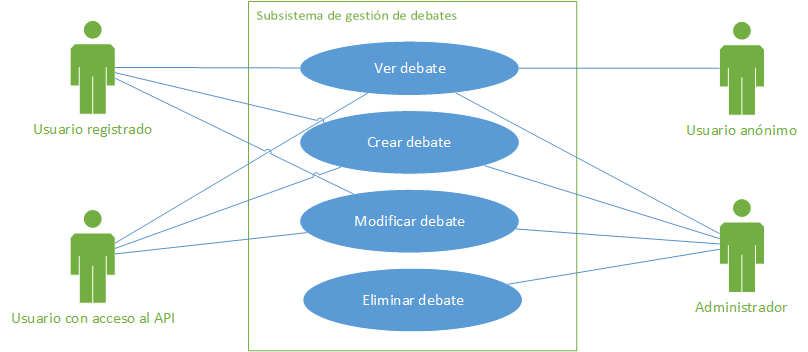
\includegraphics[width=\textwidth]{casos_uso_debates.png}
\caption{Diagrama de casos de uso del subsistema de gestión de debates}
\label{fig:casos_uso_subsistema_debates}
\end{figure}


\subsubsection{Caso de uso ``ver debate''}
\begin{description}
\item[Descripción] 				El usuario quiere ver el contenidos y los comentarios de un debate.
\item[Actores]					Cualquier usuario registrado o no en el sistema.
\item[Escenario principal]	 	\hfill
								\begin{enumerate}
								\item El usuario pulsa en el botón que carga la vista de los debates.
								\item Una vez en la vista de debates, elige el debate del que quiere ver sus contenidos.
								\item El usuario pulsa en el título del debate elegido.
								\item El sistema carga la vista del debate mostrando tanto el contenido como los comentarios del mismo.
								\end{enumerate}
\item[Escenario alternativo 1]	El usuario utiliza la búsqueda para localizar el debate.
								\begin{enumerate}
								\item El usuario accede a la vista de la búsqueda.
								\item El usuario escribe algunas palabras que se encuentren en el debate que quiere visualizar.
								\item En la lista de resultados selecciona el debate que desee.
								\item Se continua desde el punto 4 del escenario principal.
								\end{enumerate}
\end{description}


\subsubsection{Caso de uso ``crear debate''}
\begin{description}
\item[Descripción] El usuario quiere crear un nuevo debate para que puedan participar el resto de usuarios.
\item[Actores] Administrador, usuario registrado o usuario con capacidad de acceso al API.
\item[Precondiciones] Haber iniciado sesión en el sistema.
\item[Escenario principal] \hfill
						 	\begin{enumerate}
							\item El usuario accede a la vista de debates.
							\item Pulsa el botón para crear un debate.
							\item Rellena los campos requeridos en el formulario de creación del debate.
							\item Rellena los campos opcionales que considere necesarios en el formulario de creación del debate.
							\item Pulsa el botón para guardar el debate.
							\item El sistema guarda el debate con estado ``próximamente''.
							\end{enumerate}
\item[Escenario alternativo 1] El usuario no ha rellenado todos los campos requeridos.
							\begin{enumerate}
							\item El sistema notificará al usuario de que faltan campos por rellenar.
							\item Se continuará desde el punto 3 del escenario principal.
							\end{enumerate}
\end{description}


\subsubsection{Caso de uso ``comentar un debate''}
\begin{description}
\item[Descripción] El usuario quiere crear dar su opinión en un debate abierto.
\item[Actores] Administrador, usuario registrado o usuario con capacidad de acceso al API.
\item[Precondiciones] Haber iniciado sesión en el sistema.
\item[Escenario principal] \hfill
						 	\begin{enumerate}
							\item El usuario accede a la vista de debates.
							\item Selecciona el debate en el que quiere crear un comentario.
							\item Una vez en la vista del debate, el usuario escribe su comentario.
							\item Pulsa el botón de para guardar su comentario.
							\end{enumerate}
\item[Escenario alternativo 1] El usuario quiere añadir un comentario como respuesta a otro comentario ya existente.
							\begin{enumerate}
							\item Los dos primeros pasos serán similares a los del escenario principal.
							\item Una vez en la vista de debate el usuario localiza el comentario al que quiere responder y pulsa el botón correspondiente.
							\item El usuario escribe su comentario.
							\item Pulsa el botón para guardar el comentario.
							\end{enumerate}
\end{description}


\subsubsection{Caso de uso ``modificar comentario''}
\begin{description}
\item[Descripción] El usuario quiere crear modificar un comentario que ha creado previamente.
\item[Actores] Administrador, usuario registrado o usuario con capacidad de acceso al API.
\item[Precondiciones] Haber iniciado sesión en el sistema.
\item[Escenario principal] \hfill
						 	\begin{enumerate}
							\item El usuario accede a la vista de debates.
							\item Selecciona el debate en el que ha realizado el comentario que quiere modificar.
							\item Una vez en la vista del debate busca su comentario y pulsa el botón destinado a modificarlo.
							\item Introduce el nuevo texto del comentario
							\item Pulsa el botón de para guardar su comentario.
							\end{enumerate}
\end{description}


\subsubsection{Caso de uso ``moodificar debate''}
\begin{description}
\item[Descripción] Un usuario quiere modificar el contenido de un debate.
\item[Actores] Administrador, usuario registrado o usuario con capacidad de acceso al API.
\item[Precondiciones] Haber iniciado sesión en el sistema.
\item[Escenario principal] \hfill
						 	\begin{enumerate}
							\item El usuario accede a la vista de debates.
							\item Selecciona el debate cuyo contenido desea modificar.
							\item Una vez en la vista del debate pulsa el botón destinado a modificarlo.
							\item Modifica la información que sea necesaria (excepto el estado del debate, el proceso de modificación del estado de un debate está descrito en el escenario alternativo 1).
							\item Pulsa el botón de para guardar las modificaciones.
							\item El sistema actualiza los contenidos del debate.
							\end{enumerate}
\item[Escenario alternativo 1]  Modificar el estado de un debate.
							\begin{enumerate}
							\item El administrador accede al panel de administración.
							\item Selecciona el debate que desea modificar y pulsa el botón correspondiente.
							\item En la vista de edición del debate selecciona el nuevo estado que desea asignarle.
							\item Se continúa desde el punto 5 del escenario principal.
							\end{enumerate}
\item[Escenario alternativo 2]  No se rellenan todos los campos requeridos
							\begin{enumerate}
							\item El sistema informa al usuario del error y no modifica la información almacenada.
							\item Se continúa desde el punto 4 del escenario principal.
							\end{enumerate}
\end{description}


\subsubsection{Caso de uso ``eliminar debate''}
\begin{description}
\item[Descripción] El administrador quiere eliminar un debate junto con todos sus comentarios.
\item[Actores] Administrador.
\item[Precondiciones] Haber iniciado sesión en el sistema.
\item[Escenario principal] \hfill
						 	\begin{enumerate}
							\item El administardor accede a la vista de administración.
							\item Localiza el debate que desea eliminar y pulsa el botón correspondiente.
							\item El debate y sus comentarios serán eliminados del sistema.
							\end{enumerate}
\end{description}

\subsection{Subsistema de gestión de eventos}
\label{casos_uso_subsistema_eventos}
En esta sección se detallarán los casos de uso pertenecientes al subsistema de gestión de eventos. La figura \ref{fig:casos_uso_subsistema_eventos} muestra el diagrama de casos de uso de dicho subsistema.

\begin{figure}[h]
\centering
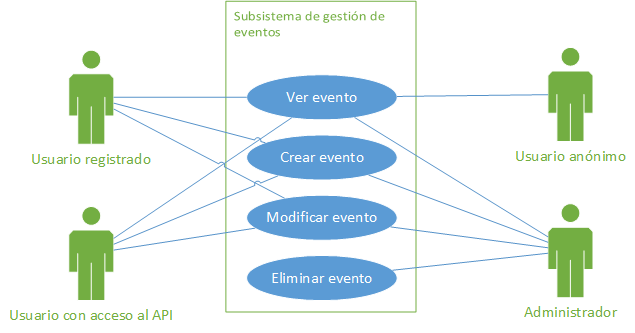
\includegraphics[width=\textwidth]{casos_uso_eventos}
\caption{Diagrama de casos de uso del subsistema de gestión de eventos}
\label{fig:casos_uso_subsistema_eventos}
\end{figure}


\subsubsection{Caso de uso ``ver evento''}
\begin{description}
\item[Descripción] Un usuario quiere ver el contenido de un evento.
\item[Actores] Cualquier usuario registrado o no en el sistema.
\item[Escenario principal] 	\hfill
							\begin{enumerate}
							\item El usuario accede a la vista de eventos.
							\item Una vez en la vista de eventos, elige el evento del que quiere ver sus contenidos.
							\item Pulsa en el título del evento que quiere ver en detalle.
							\item El sistema carga la vista del evento mostrando todos sus detalles.
							\end{enumerate}
\end{description}


\subsubsection{Caso de uso ``crear evento''}
\begin{description}
\item[Descripción]  Un usuario quiere añadir un nuevo evento al sistema.
\item[Actores]  Administrador, usuario registrado o usuario con capacidad de acceso al API.
\item[Precondiciones] Haber iniciado sesión en el sistema.
\item[Escenario principal]  \hfill
							\begin{enumerate}
							\item El usuario accede a la vista de los eventos.
							\item Una vez en la vista de eventos pulsa el botón correspondiente para crear un evento nuevo.
							\item Rellena el formulario con los datos requeridos.
							\item Si lo desea también rellena la información opcional del formulario.
							\item El usuario pulsa el botón guardar, y el sistema crea el nuevo evento.
							\end{enumerate}
\item[Escenario alternativo 1] No se han rellenado todos los campos requeridos.
							\begin{enumerate}
							\item El usuario no ha rellenado todos los campos requeridos para crear un nuevo evento.
							\item El sistema notificará al usuario de su error y no creará el nuevo evento.
							\item Se continuará desde el punto 3 del escenario principal.
							\end{enumerate}
\end{description}


\subsubsection{Caso de uso ``modificar evento''}
\begin{description}
\item[Descripción]  Un usuario quiere modificar un evento del sistema.
\item[Actores]  Administrador, usuario registrado o usuario con capacidad de acceso al API.
\item[Precondiciones]  Haber iniciado sesión en el sistema.
\item[Escenario principal]	\hfill
							\begin{enumerate}
							\item El usuario accede a la vista de los eventos..
							\item Una vez en la vista de eventos localiza el evento que quiere modificar.
							\item Cuando ha accedido al evento pulsa el botón correspondiente para modificar su contenido.
							\item Rellena toda la información requerida en el formulario.
							\item Si lo desea también rellena la información opcional del formulario.
							\item El usuario pulas el botón guardar y el sistema modifica la información del evento.
							\end{enumerate}
\item[Escenario alternativo 1] No se han rellenado todos los campos requeridos.
							\begin{enumerate}
							\item El usuario no ha rellenado todos los campos requeridos para modificar el evento.
							\item El sistema notificará al usuario de su error y no modificará los datos del evento.
							\item Se continuará desde el punto 4 del escenario principal.
							\end{enumerate}
\end{description}


\subsubsection{Caso de uso ``eliminar evento''}
\begin{description}
\item[Descripción]  Un administrador quiere eliminar un evento del sistema.
\item[Actores] El administrador del sistema.
\item[Precondiciones]  Haber iniciado sesión en el sistema.
\item[Escenario principal]	\hfill
							\begin{enumerate}
							\item El administrador accede a la vista de administración.
							\item Localiza el evento que desea eliminar y pulsa el botón correspondiente.
							\item El evento será eliminado del sistema.
							\end{enumerate}
\end{description}

\subsection{Subsistema de gestión de noticias}
\label{casos_uso_subsistema_noticias}
En esta sección se detallarán los casos de uso pertenecientes al subsistema de gestión de noticias. La figura \ref{fig:casos_uso_subsistema_noticias} muestra el diagrama de casos de uso de dicho subsistema.

\begin{figure}[h]
\centering
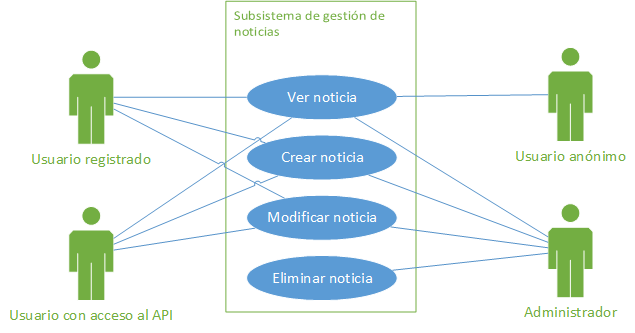
\includegraphics[width=\textwidth]{casos_uso_noticias}
\caption{Diagrama de casos de uso del subsistema de gestión de noticias}
\label{fig:casos_uso_subsistema_noticias}
\end{figure}


\subsubsection{Caso de uso ``ver noticia''}
\begin{description}
\item[Descripción] Un usuario quiere ver el contenido de una noticia.
\item[Actores] Cualquier usuario registrado o no en el sistema.
\item[Escenario principal] 	\hfill
							\begin{enumerate}
							\item El usuario pulsa en el botón que carga la vista de las noticias.
							\item Una vez en la vista de noticias pulsa en el título de la noticia que quiere ver en detalle.
							\item El sistema carga la vista de la noticia mostrando todos sus detalles.
							\end{enumerate}
\end{description}


\subsubsection{Caso de uso ``crear noticia''}
\begin{description}
\item[Descripción]  Un usuario quiere añadir una nueva noticia al sistema.
\item[Actores]  Administrador, usuario registrado o usuario con capacidad de acceso al API.
\item[Precondiciones] Haber iniciado sesión en el sistema.
\item[Escenario principal]  \hfill
							\begin{enumerate}
							\item El usuario pulsa en el botón que carga la vista de las noticias.
							\item Una vez en la vista de las noticias pulsa el botón correspondiente para crear una noticia nueva.
							\item Rellena el formulario con los datos requeridos.
							\item Si lo desea también rellena la información opcional del formulario.
							\item El usuario pulsa el botón guardar.
							\item El sistema crea la nueva noticia.
							\end{enumerate}
\item[Escenario alternativo 1] No se han rellenado todos los campos requeridos.
							\begin{enumerate}
							\item El usuario no ha rellenado todos los campos requeridos para crear una nueva noticia.
							\item El sistema notificará al usuario de su error y no creará la nueva noticia.
							\item Se continuará desde el punto 3 del escenario principal.
							\end{enumerate}
\end{description}


\subsubsection{Caso de uso ``modificar noticia''}
\begin{description}
\item[Descripción]  Un usuario quiere modificar una noticia del sistema.
\item[Actores]  Administrador, usuario registrado o usuario con capacidad de acceso al API.
\item[Precondiciones]  Haber iniciado sesión en el sistema.
\item[Escenario principal]	\hfill
							\begin{enumerate}
							\item El usuario accede a la vista de las noticias.
							\item Una vez en la vista de noticias localiza la noticia que quiere modificar.
							\item Cuando ha accedido a la noticia pulsa el botón correspondiente para modificar su contenido.
							\item Rellena toda la información requerida en el formulario.
							\item Si lo desea también rellena la información opcional del formulario.
							\item El usuario pulas el botón guardar.
							\item El sistema actualiza la información de la noticia editada.
							\end{enumerate}
\item[Escenario alternativo 1] No se han rellenado todos los campos requeridos.
							\begin{enumerate}
							\item El usuario no ha rellenado todos los campos requeridos para modificar la noticia.
							\item El sistema notificará al usuario de su error y no modificará los datos la noticia.
							\item Se continuará desde el punto 4 del escenario principal.
							\end{enumerate}
\end{description}


\subsubsection{Caso de uso ``eliminar noticia''}
\begin{description}
\item[Descripción]  Un administrador quiere eliminar una noticia del sistema.
\item[Actores]  El administrador del sistema.
\item[Precondiciones]  Haber iniciado sesión en el sistema.
\item[Escenario principal]	\hfill
							\begin{enumerate}
							\item El administrador accede a la vista de administración.
							\item Localiza la noticia que desea eliminar y pulsa el botón correspondiente.
							\item La noticia será eliminado del sistema.
							\end{enumerate}
\end{description}

\subsection{Subsistema de gestión de entradas del blog}
\label{casos_uso_subsistema_blog}
En esta sección se detallarán los casos de uso y escenarios pertenecientes al subsistema de gestión de entradas del blog. La figura \ref{fig:casos_uso_subsistema_blog} muestra el diagrama de casos de uso del subsistema de gestión de debates.

\begin{figure}[h]
\centering
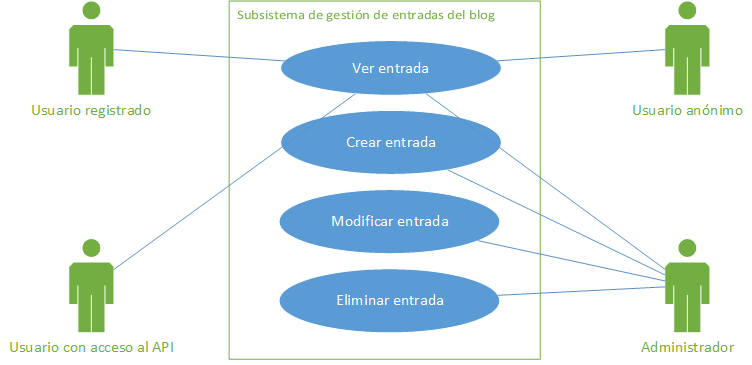
\includegraphics[width=\textwidth]{casos_uso_blog}
\caption{Diagrama de casos de uso del subsistema de gestión de entradas del blog}
\label{fig:casos_uso_subsistema_blog}
\end{figure}


\subsubsection{Caso de uso ``ver entrada''}
\begin{description}
\item[Descripción] 				El usuario quiere ver el contenido de una entrada del blog.
\item[Actores]					Cualquier rol de usuario.
\item[Escenario principal]	 	\hfill
								\begin{enumerate}
								\item El usuario accede al blog del Land Portal.
								\item Una vez en el blog, selecciona la entrada que quiere ver en detalle.
								\item El sistema carga la vista de la entrada mostrando tanto su contenido como sus comentarios.
								\end{enumerate}
\end{description}


\subsubsection{Caso de uso ``crear entrada''}
\begin{description}
\item[Descripción] El administrador quiere crear una nueva entrada en el blog del Land Portal.
\item[Actores] Administrador.
\item[Precondiciones] Haber iniciado sesión en el sistema.
\item[Escenario principal] \hfill
						 	\begin{enumerate}
							\item El administrador accede al blog del Land Portal.
							\item Una vez en el blog, el administrador pulsa el botón para crear una nueva entrada.
							\item Rellena los campos requeridos en el formulario de creación de la entrada.
							\item Rellena los campos opcionales que considere necesarios en el formulario de creación de la entrada.
							\item Pulsa el botón para guardar la entrada.
							\item El sistema guarda la entrada y la hace visible para todos los usuarios en el blog.
							\end{enumerate}
\item[Escenario alternativo 1] El administrador no ha rellenado todos los campos requeridos.
							\begin{enumerate}
							\item El sistema notificará al usuario de que faltan campos por rellenar.
							\item Se continuará desde el punto 3 del escenario principal.
							\end{enumerate}
\end{description}


\subsubsection{Caso de uso ``modificar entrada''}
\begin{description}
\item[Descripción] El administrador quiere modificar el contenido de una entrada del blog.
\item[Actores] El administrador del sistema.
\item[Precondiciones] Haber iniciado sesión en el sistema.
\item[Escenario principal] \hfill
						 	\begin{enumerate}
							\item El administrador accede al blog del Land Portal.
							\item Una vez en el blog, el administrador selecciona la entrada que quiere modificar.
							\item En la entrada correspondiente, el administrador pulsa el botón para editar su contenido.
							\item Rellena los campos requeridos en el formulario de modificación de la entrada.
							\item Rellena los campos opcionales que considere necesarios en el formulario de modificación de la entrada.
							\item Pulsa el botón para guardar los cambios
							\item El sistema actualiza los contenidos de la entrada del blog.
							\end{enumerate}
\item[Escenario alternativo 1]  No se rellenan todos los campos requeridos
							\begin{enumerate}
							\item El sistema informa al usuario del error y no modifica la información almacenada.
							\item Se continúa desde el punto 4 del escenario principal.
							\end{enumerate}
\end{description}

\subsubsection{Caso de uso ``eliminar entrada''}
\begin{description}
\item[Descripción] El administrador quiere eliminar una entrada del blog junto con todos sus comentarios.
\item[Actores] El administrador del sistema.
\item[Precondiciones] Haber iniciado sesión en el sistema.
\item[Escenario principal] \hfill
						 	\begin{enumerate}
							\item El administrador accede a la vista de administración.
							\item En la sección de contenidos localiza la entrada y pulsa el botón correspondiente para eliminarla.
							\item La entrada y sus comentarios serán eliminados del sistema.
							\end{enumerate}
\end{description}



\subsection{Subsistema de gestión de comentarios}
\label{casos_uso_subsistema_comentarios}
En esta sección se detallarán los casos de uso y escenarios pertenecientes al subsistema de gestión de comentarios. La figura \ref{fig:casos_uso_subsistema_comentarios} muestra el diagrama de casos de uso de dicho subsistema.

\begin{figure}[h]
\centering
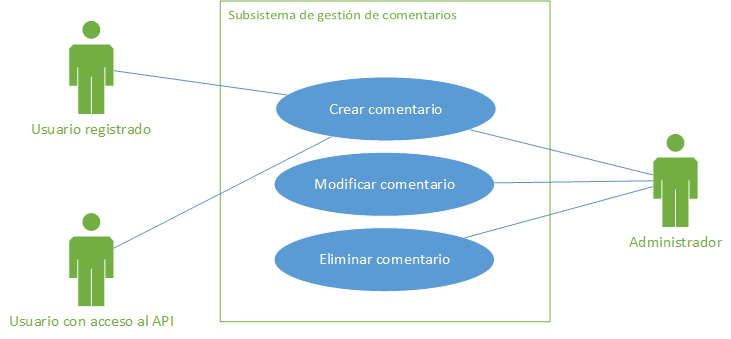
\includegraphics[width=\textwidth]{casos_uso_comentarios}
\caption{Diagrama de casos de uso del subsistema de gestión de comentarios}
\label{fig:casos_uso_subsistema_comentarios}
\end{figure}


\subsubsection{Caso de uso ``crear comentario''}
\begin{description}
\item[Descripción] El usuario quiere crear un nuevo comentario.
\item[Actores] Administrador, usuario registrado o usuario con capacidad de acceso al API.
\item[Precondiciones] Haber iniciado sesión en el sistema.
\item[Escenario principal] \hfill
						 	\begin{enumerate}
							\item El usuario accede a la entrada del blog o al debate en el que quiere crear el comentario.
							\item El usuario escribe su comentario.
							\item Pulsa el botón de para guardar su comentario.
							\item El sistema guarda el comentario y lo hace visible al resto de usuarios.
							\end{enumerate}
\item[Escenario alternativo 1] Comentario en un  debate cerrado.
							\begin{enumerate}
							\item El usuario accede al debate en el que quiere crear el comentario.
							\item El sistema no mostrará opciones para que el usuario cree un comentario.
							\end{enumerate}
\end{description}


\subsubsection{Caso de uso ``modificar comentario''}
\begin{description}
\item[Descripción] El administrador desea modificar el contenido de un comentario realizado por un usuario.
\item[Actores] Administrador.
\item[Precondiciones] Haber iniciado sesión en el sistema.
\item[Escenario principal] \hfill
						 	\begin{enumerate}
							\item El usuario accede a la entrada del blog o al debate en el que se encuentra el comentario a modificar.
							\item El administrador localiza el comentario y pulsa el botón modificar.
							\item El administrador introduce el texto que crea conveniente y pulsa el botón guardar.
							\item El sistema actualiza el contenido del comentario modificado.
							\end{enumerate}
\end{description}


\subsubsection{Caso de uso ``eliminar comentario''}
\begin{description}
\item[Descripción] El administrador desea eliminar un comentario realizado por un usuario.
\item[Actores] Administrador.
\item[Precondiciones] Haber iniciado sesión en el sistema.
\item[Escenario principal] \hfill
						 	\begin{enumerate}
							\item El usuario accede a la entrada del blog o al debate en el que se encuentra el comentario a eliminar.
							\item El administrador localiza el comentario y pulsa el botón eliminar.
							\item El sistema elimina el comentario y deja de mostrarlo.
							\end{enumerate}
\end{description}

\subsection{Subsistema de búsqueda}
\label{casos_uso_subsistema_busqueda}
En esta sección se detallarán los casos de uso y escenarios pertenecientes al subsistema de búsqueda. La figura \ref{fig:casos_uso_subsistema_busqueda} muestra el diagrama de casos de uso de dicho subsistema.

\begin{figure}[h]
\centering
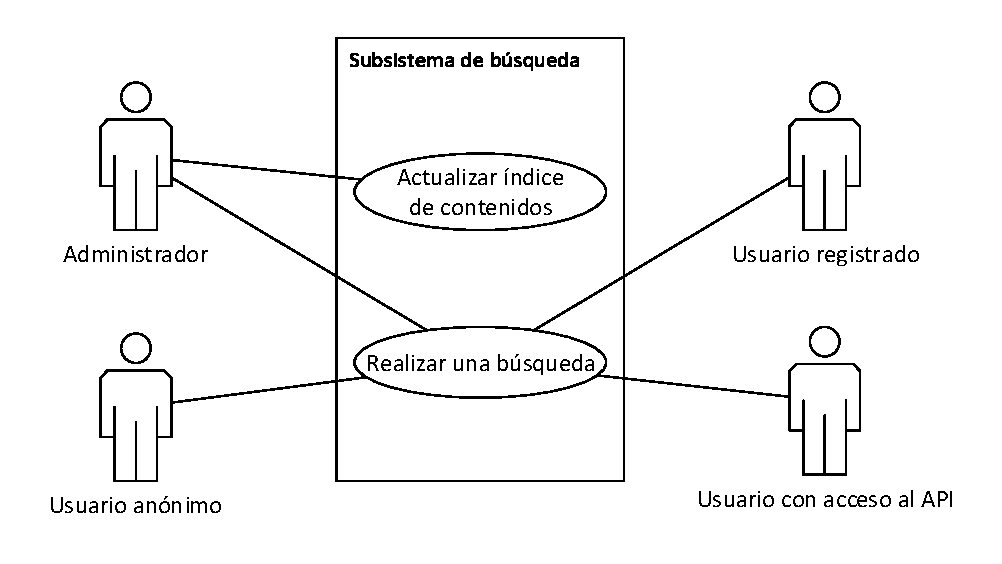
\includegraphics[width=\textwidth]{casos_uso/diagrama_casos_uso_busqueda}
\caption{Diagrama de casos de uso del subsistema de búsqueda}
\label{fig:casos_uso_subsistema_busqueda}
\end{figure}

\subsubsection{Caso de uso ``realizar una búsqueda''}
\begin{description}
\item[Descripción] Un usuario busca información en el sistema.
\item[Actores] Cualquier rol de usuario registrado o no en el sistema.
\item[Escenario principal] \hfill
							\begin{enumerate}
							\item El usuario introduce un texto en el formulario de búsqueda
							\item El usuario pulsa el botón de buscar
							\item El sistema devuelve los resultados correspondientes
							\end{enumerate}						
\end{description}

\subsubsection{Caso de uso ``actualizar índice de contenidos''}
\begin{description}
\item[Descripción] El administrador actualiza el índice de contenidos del subsistema de búsqueda.
\item[Actores] El administrador del sistema.
\item[Escenario principal] \hfill
							\begin{enumerate}
							\item El administrador accede al panel de administración.
							\item Una vez en el panel de administración, accede a las opciones de la búsqueda
							\item El administrador pulsa el botón correspondiente para realizar la regeneración del índice de contenidos.
							\item El sistema actualiza el índice de contenidos incluyendo los nuevos contenidos y eliminado los contenidos que ya no existan.
							\end{enumerate}						
\end{description}

\subsection{Subsistema de gestión de datos}
\label{casos_uso_subsistema_datos}
En esta sección se detallarán los casos de uso pertenecientes al subsistema de datos. La figura \ref{fig:casos_uso_subsistema_datos} muestra el diagrama de casos de uso de dicho subsistema.

\begin{figure}[h]
\centering
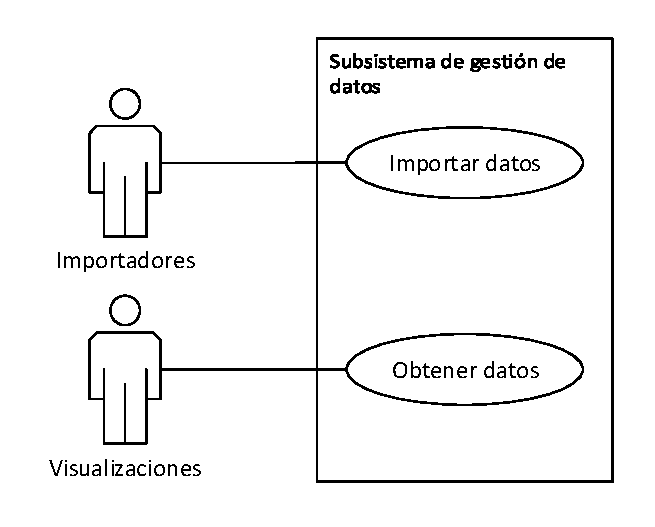
\includegraphics{casos_uso/diagrama_casos_uso_datos}
\caption{Diagrama de casos de uso del subsistema de datos}
\label{fig:casos_uso_subsistema_datos}
\end{figure}

\subsubsection{Caso de uso ``importar datos''}
\begin{description}
\item[Descripción] Un importador quiere incluir nueva información en el sistema.
\item[Actores] Un importador.
\item[Escenario principal] \hfill
							\begin{enumerate}
							\item El importador envía una petición POST al subsistema de datos incluyendo un fichero XML conforme a un XML Schema definido y con los datos a incluir en el sistema.
							\item El subsistema de datos comprueba si la dirección de origen de la petición está en la lista blanca.
							\item El subsistema de datos procesa la petición convirtiendo la información del fichero XML a un modelo propio.
							\item El subsistema de datos persiste en la base de datos el modelo creado anteriormente.
							\item El subsistema envía una respuesta 200 (\textit{OK}) al importador.
							\end{enumerate}
\item[Escenario alternativo 1] Los datos enviados por el importador no se ajustan al XML Schema.
							\begin{enumerate}
							\item El subsistema de datos no insertará ningún dato en la base de datos.
							\item El subsistema de datos envía una respuesta de error al importador.
							\end{enumerate}
\item[Escenario alternativo 2] El verbo utilizado por el importador no es el correcto (GET, PUT, etc).
							\begin{enumerate}
							\item El subsistema de datos no insertará ningún dato en la base de datos.
							\item El subsistema de datos envía una respuesta de error 405 (\textit{Method not Allowed}) al importador.
							\end{enumerate}
\item[Escenario alternativo 3] La petición realizada por el importador no incluye el fichero XML con los datos.
							\begin{enumerate}
							\item El subsistema de datos no insertará ningún dato en la base de datos.
							\item El subsistema de datos envía una respuesta de error 400 (\textit{Bad Request}) al importador.
							\end{enumerate}
\item[Escenario alternativo 4] La petición proviene de un origen no confiable
							\begin{enumerate}
							\item El subsistema de datos aborta la petición con un código de error 403 (\textit{Forbidden}).
							\end{enumerate}
\end{description}	

\subsubsection{Caso de uso ``obtener datos''}
\begin{description}
\item[Descripción] Una visualización pide datos para presentarlos al usuario de forma atractiva.
\item[Actores] Visualizaciones.
\item[Escenario principal] 	\hfill
							\begin{enumerate}
							\item La visualización lanza una petición GET al subsistema de datos.
							\item El subsistema de datos devuelve un fichero JSON con los datos correspondientes a la petición realizada.
							\item La visualización procesa los datos recibidos para presentarlos de forma visual.
							\end{enumerate}
\item[Escenario alternativo 1] La petición de la visualización es errónea.
							\begin{enumerate}
							\item La visualización lanza una petición al subsistema de datos.
							\item El subsistema de datos responde con un código de error HTTP.
							\end{enumerate}
\end{description}